\section{Resultados}
Despues de realizar el experimento el script the python nos arrojo las siguientes graficas:
\begin{figure}[H]
    \centering   
    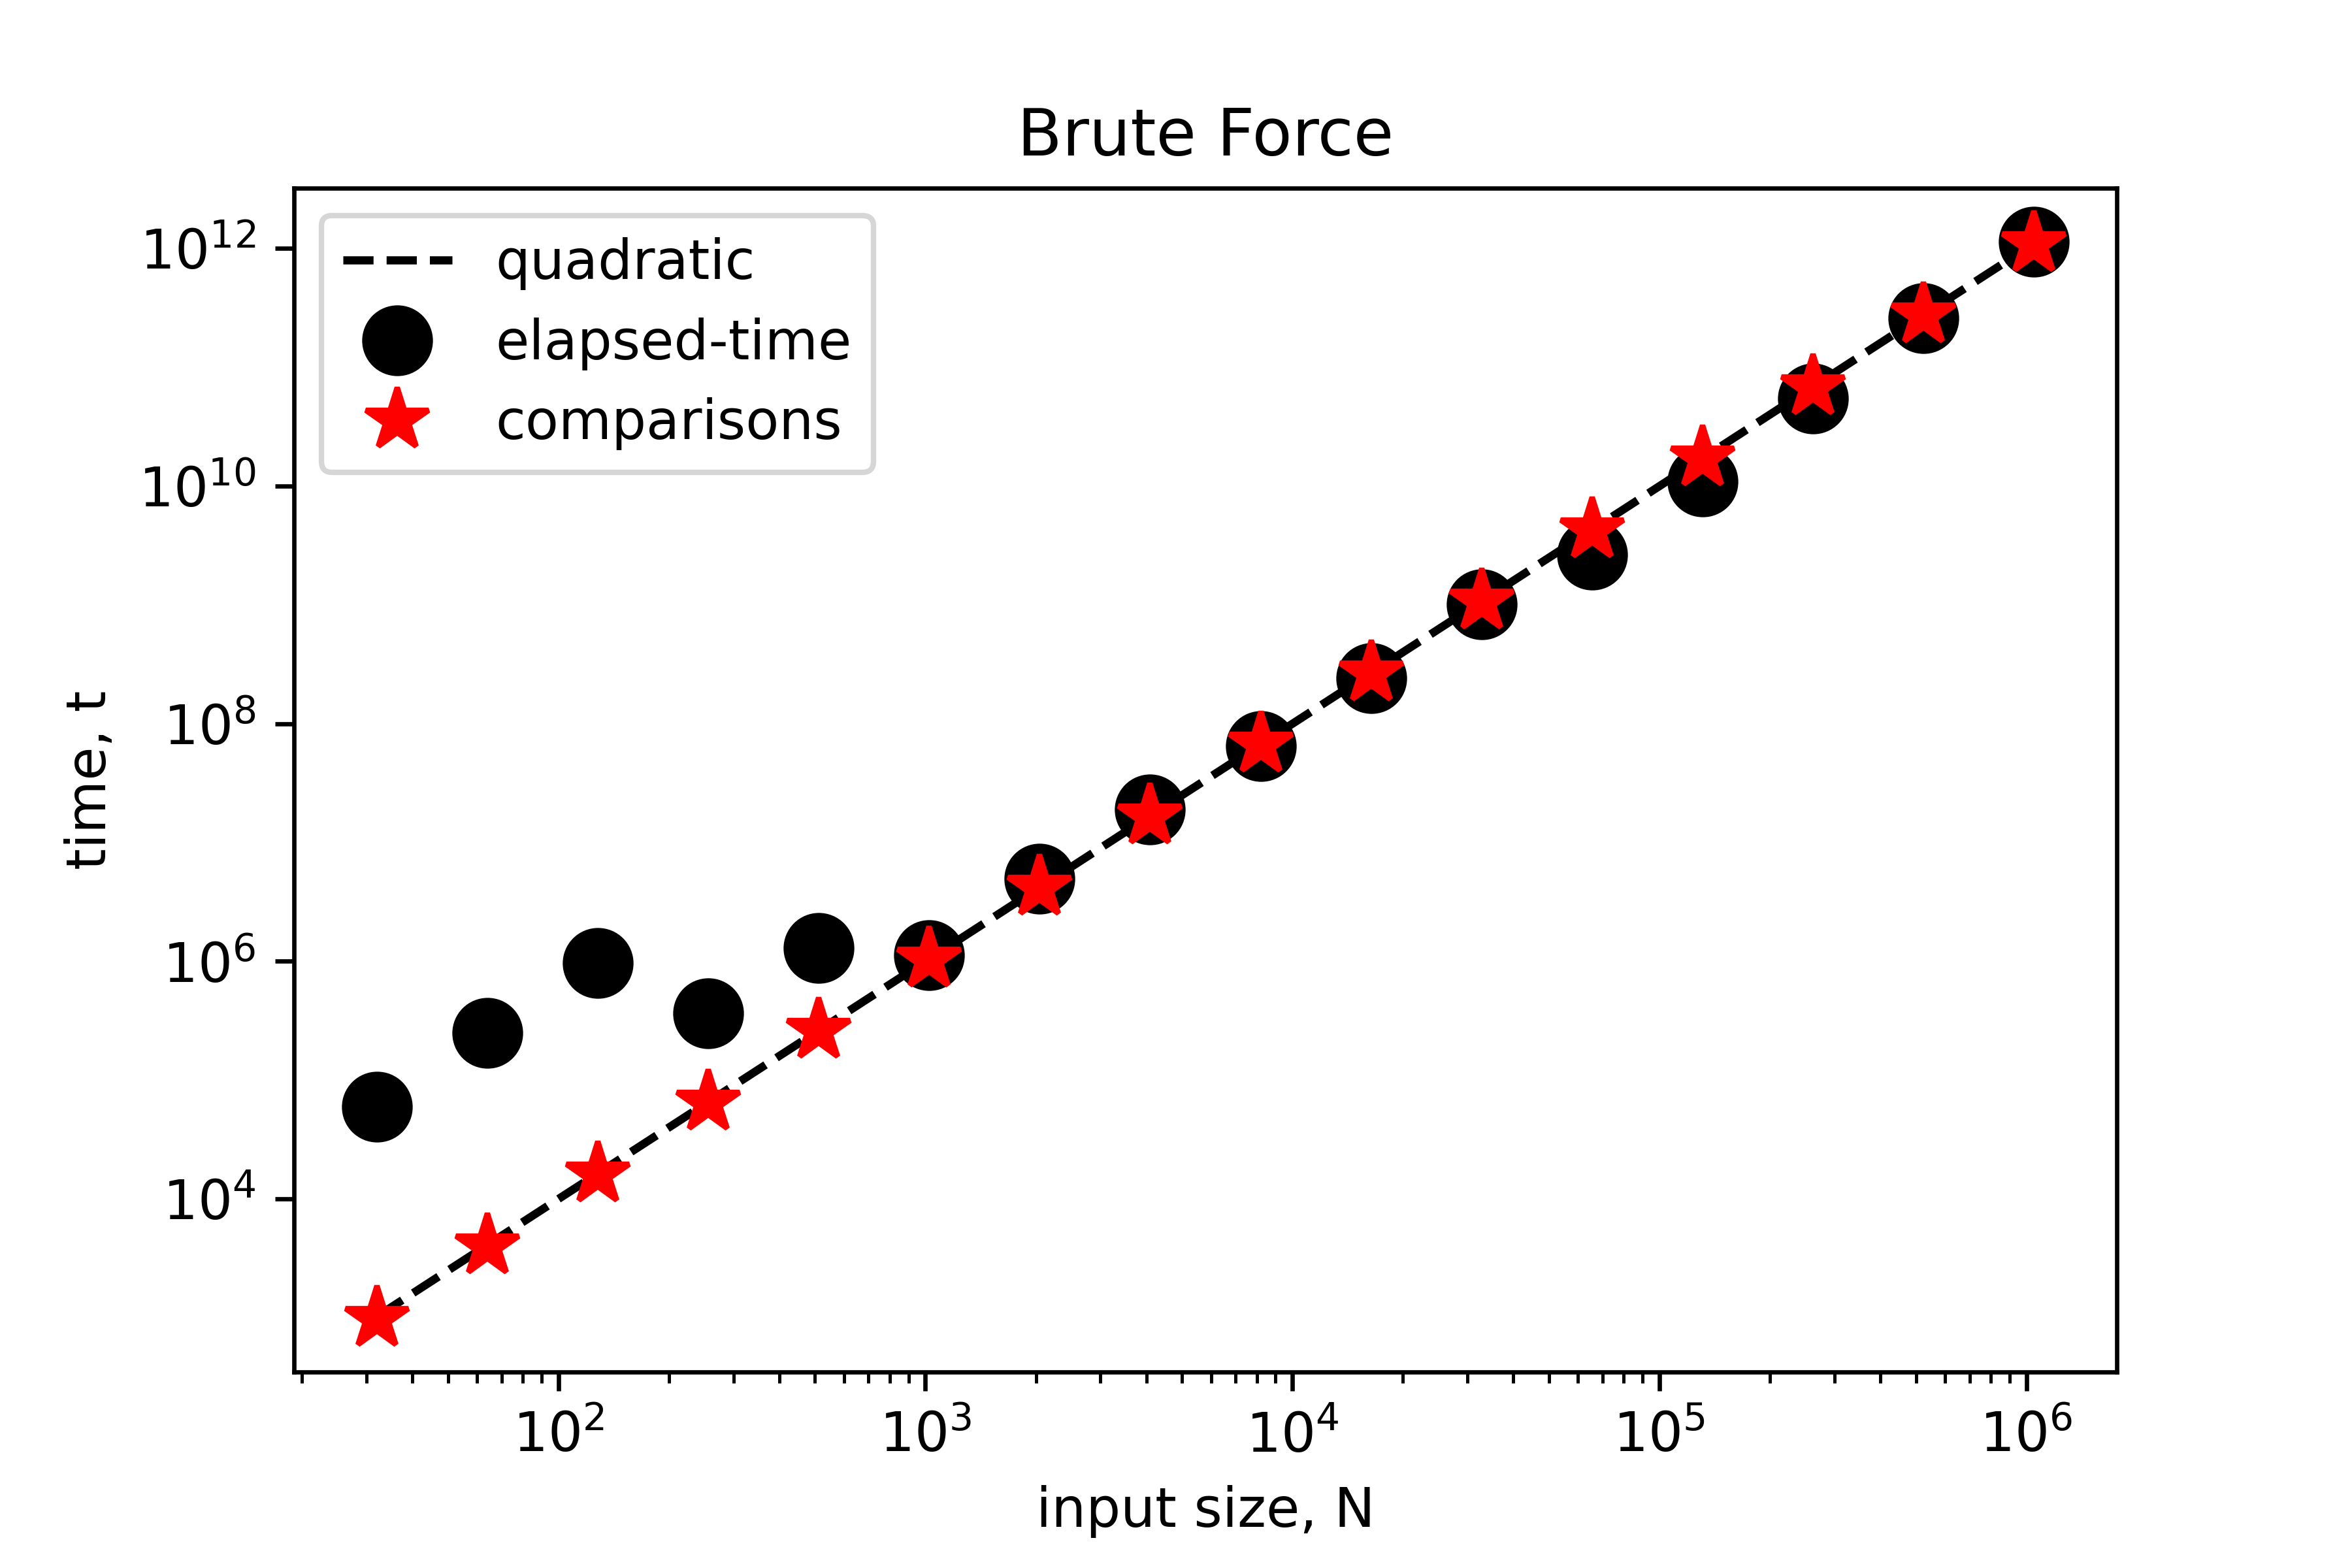
\includegraphics[width=0.45\textwidth,\keepaspectratio]{Images/Brute.png}
    \caption{Comportamiento de la tecnica de Fuerza bruta}
\end{figure}%

\begin{figure}[H]
    \centering    
    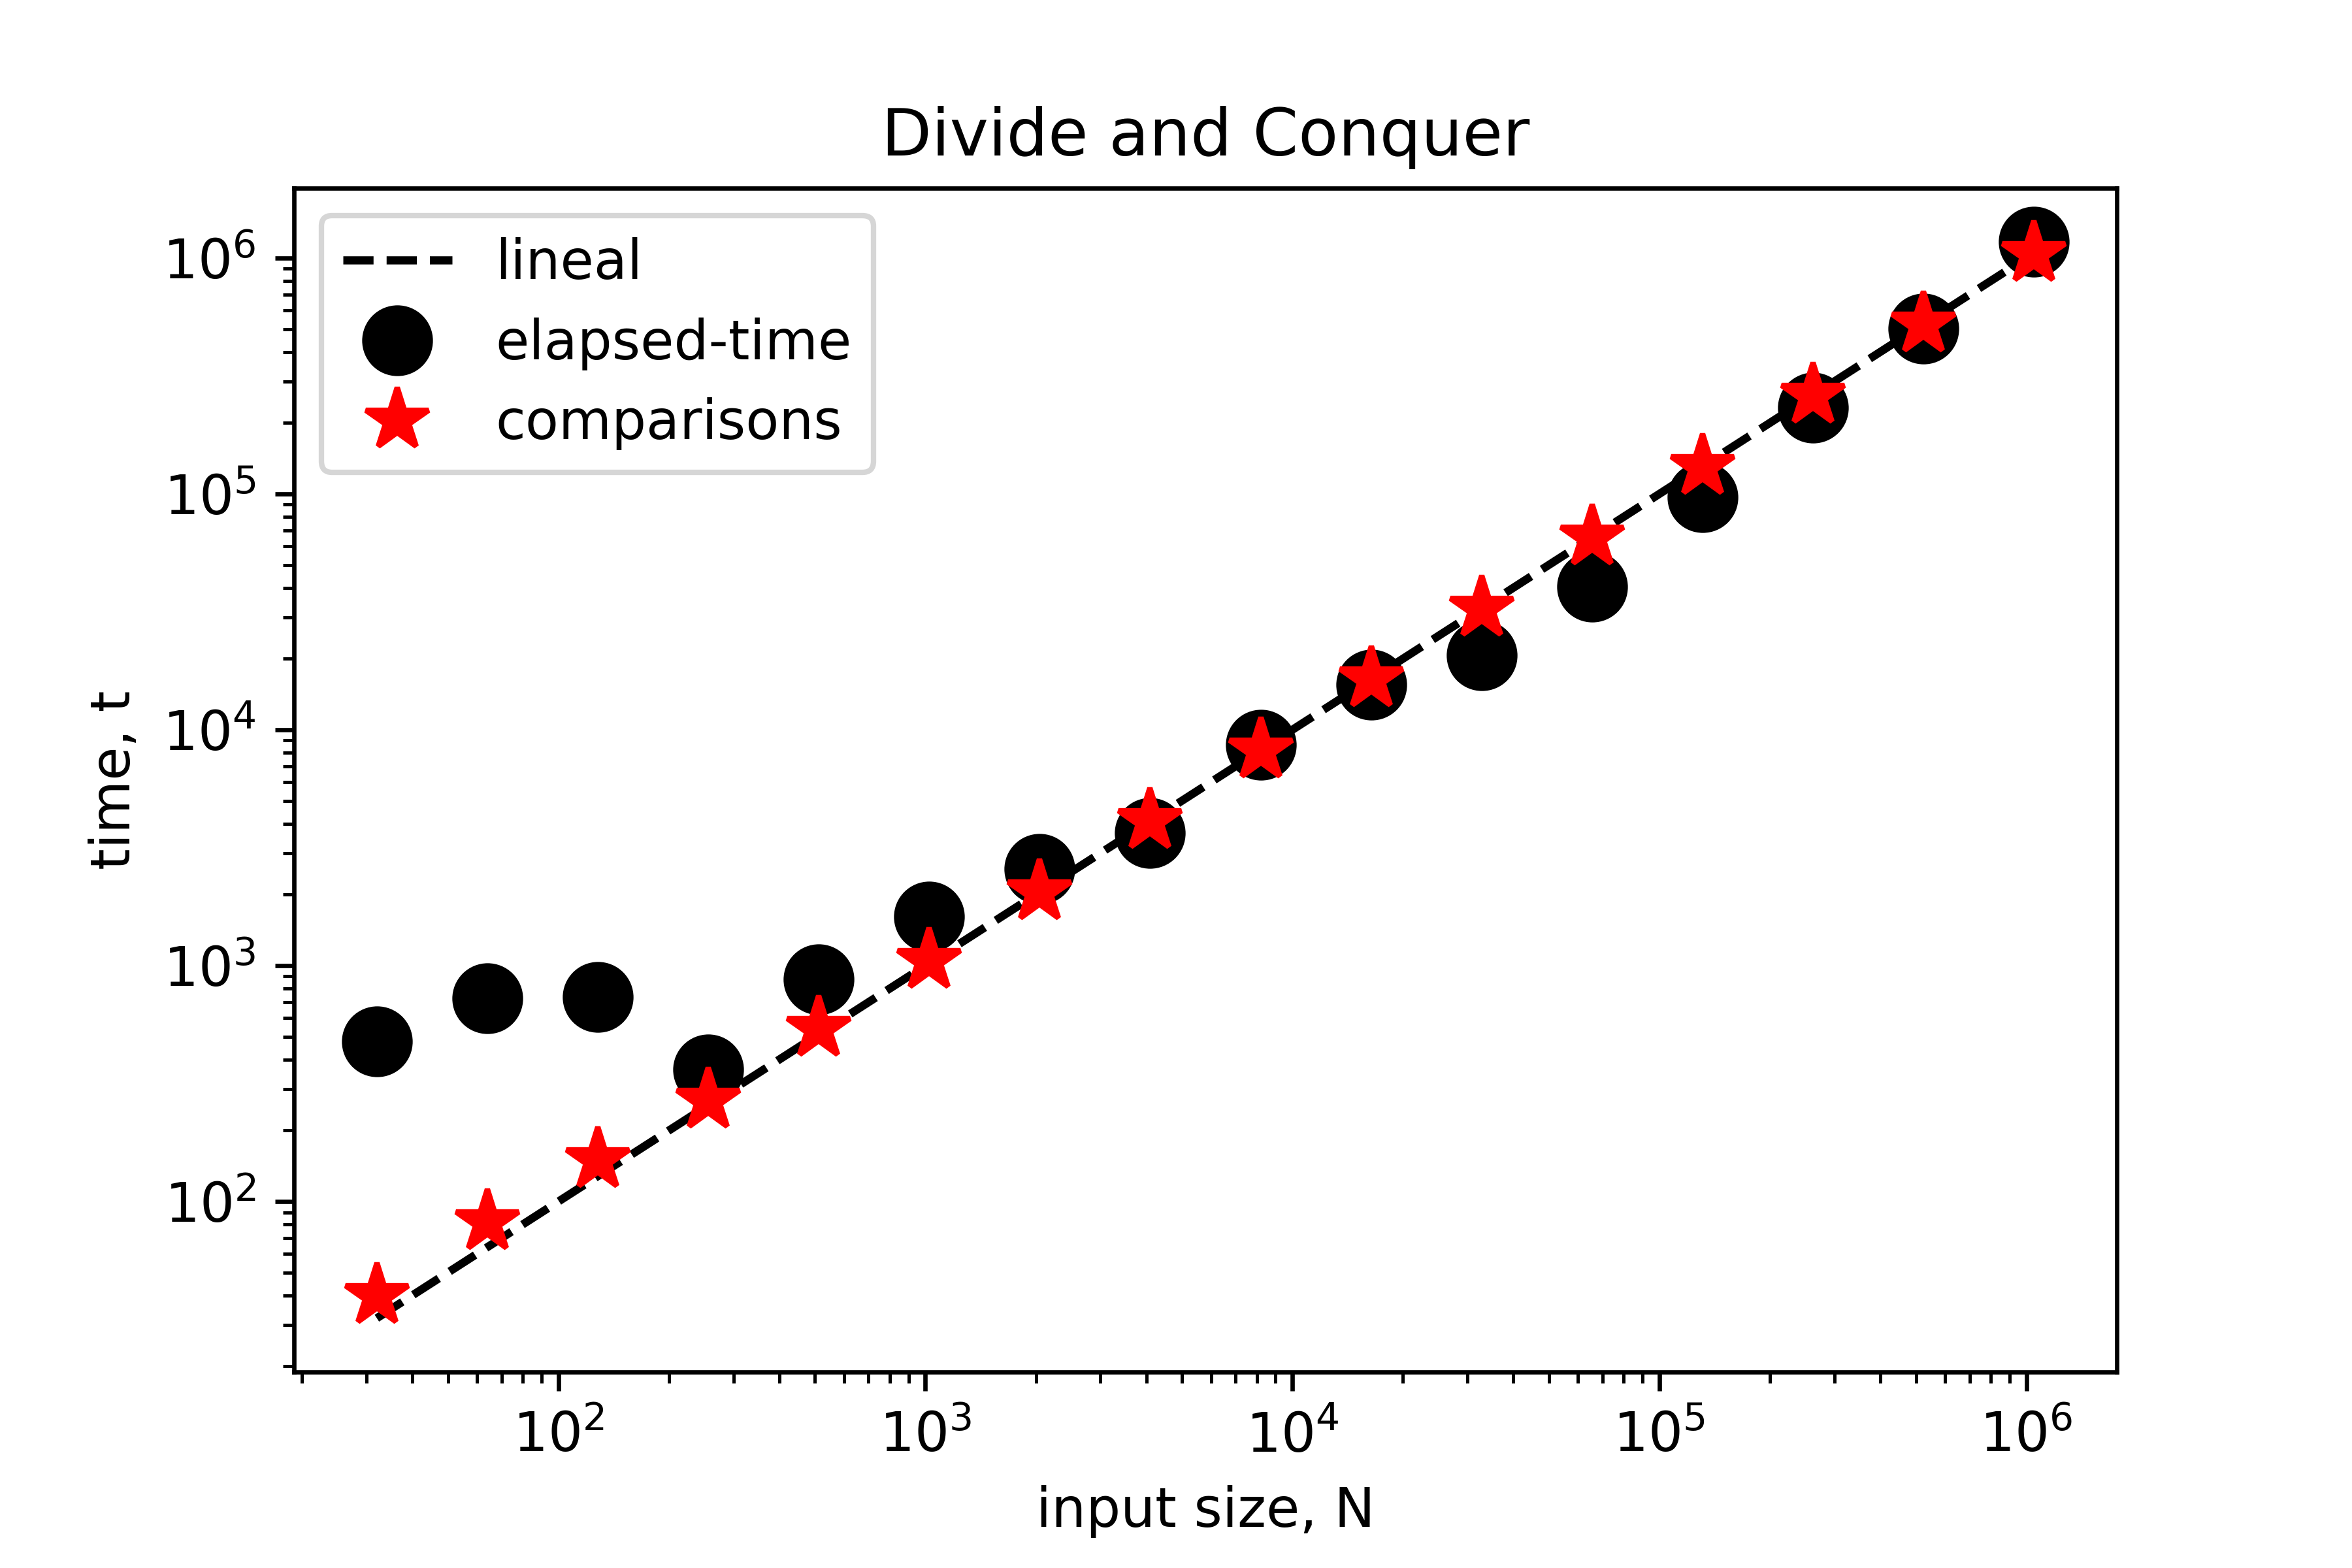
\includegraphics[width=0.45\textwidth,\keepaspectratio]{Images/Divide.png}
    \caption{Comportamiento de la tecnica de Divide y Venceras}
\end{figure}%

Observando las gráficas podemos notar que usando la técnica de “divide y vencerás” la complejidad temporal crece de manera lineal $O(N)$, aunque no de manera totalmente precisa, pues el número de iteraciones depende de la lista de coordenadas, por lo que los datos no están alineados en su totalidad al ajuste lineal, aunque se comportan de manera parecida. Por otro lado, la técnica de “fuerza bruta” tiene una complejidad temporal de $O(N^2)$, es decir que aumenta de manera exponencial, y sin importar los datos del arreglo el número de iteraciones dado un mismo N será el mismo y se ajusta de manera perfecta al ajuste exponencial. La diferencia está en que usando la técnica de “divide y vencerás”, el programa no compara cada par de puntos en la lista, sino que compara solo los que están más cercanos, lo que ahorra una gran cantidad de comparaciones, lo que hace que el número de iteraciones aumenten de manera parecida a N, es decir de manera lineal. Sin embargo, usando la técnica de “fuerza bruta”, sin importar que las coordenadas estén muy lejanas se calcula la distancia entre ellas, lo que hace que se tengan que realizar muchas más comparaciones de las necesarias, y provocan que el número de iteraciones aumenten de manera exponencial a medida que aumente N.